% BANKS-SOURCE: pdf=191 print=181 kind=section id=9.11
\subsection{Coupling renormalization in non-abelian gauge theory}

The physical gauge theory in this section has $D=4$ space-time dimensions.
Dimensional regularization uses $d_{\mathrm{reg}}$ for the continued loop
dimension.  For the static configuration, $\mathbf R$ is the source
separation and $R=|\mathbf R|$.

% BANKS-SOURCE: pdf=191 print=181 kind=source-page
% BANKS-SOURCE: pdf=191 print=181 kind=prose
We will calculate the renormalization of the coupling by computing the one-loop
correction to the potential between two static external sources. As explained
in Chapter 8 and Problem 8.4, this potential is defined by
% BANKS-SOURCE: pdf=191 print=181 kind=equation id=9.2
\begin{equation}
  V(R)=-\lim_{T\to\infty}\frac{1}{T}\ln\langle W_R(\Gamma)\rangle/d_R.
  \label{eq:9.2}
\end{equation}
$\Gamma$ is the rectangular Wilson loop shown in Figure~\ref{fig:9.8} and
$d_R$ is the dimension of the representation $R$.

In perturbation theory we can compute this in terms of the Feynman rules of
Appendix D, with additional vertices for the interaction of gluons,\footnote[16]{We
will use the QCD terminology, \emph{gluon}, to refer to the generic non-abelian
gauge bosons of this section.} and the static source. The contributions
proportional to $T$ come exclusively from the parts of the Wilson loop which
point in the Euclidean time direction. Thus we have
% BANKS-SOURCE: pdf=191 print=181 kind=display
\[
  g_0\mu^{(4-d_{\mathrm{reg}})/2}\delta_{\mu0}
  \delta^3(\mathbf x-\mathbf R)T_R^a,
\]
for the upward-going line at $R$, and
% BANKS-SOURCE: pdf=191 print=181 kind=display
\[
  -g_0\mu^{(4-d_{\mathrm{reg}})/2}\delta_{\mu0}
  \delta^3(\mathbf x)T_R^a,
\]
for the downward-going line at the origin. We will work in Feynman gauge,
because the triple gluon vertex of Figure~\ref{fig:9.9}(f) will not contribute
in this gauge. All the gluons couple to static sources, so only their $0$
components appear. The triple vertex is anti-symmetric in group indices (we
have a compact group) and in space indices (Bose statistics), and so vanishes
in this configuration.

% BANKS-SOURCE: pdf=191 print=181 kind=figure id=9.8
\begin{figure}[htbp]
  \centering
  % BANKS-SOURCE: pdf=191 print=181 kind=figure id=9.8
\begin{tikzpicture}[x=1cm,y=1cm,baseline=-.4ex]
  % rectangular Wilson loop, traversed counter-clockwise:
  % right along the bottom, up the right edge, left along the top, down the left edge
  \draw[line width=.55pt,
        decoration={markings,
          mark=at position 0.092  with {\arrow{Latex[length=2.4mm,width=2.4mm]}},
          mark=at position 0.3333 with {\arrow{Latex[length=2.4mm,width=2.4mm]}},
          mark=at position 0.592  with {\arrow{Latex[length=2.4mm,width=2.4mm]}},
          mark=at position 0.8333 with {\arrow{Latex[length=2.4mm,width=2.4mm]}}},
        postaction={decorate}]
    (-1,-2) -- (1,-2) -- (1,2) -- (-1,2) -- cycle;
  % one-gluon exchange between the two static sources, at mid-height
  \draw[decorate,decoration={coil,aspect=.7,segment length=9pt,amplitude=5pt},
        line width=.55pt]
    (-1,0) -- (1,0);
  \node[anchor=east] at (-1.1,-2) {$0$};
  \node[anchor=west] at (1.1,-2) {$R$};
  \node[anchor=west] at (1.15,0) {$T$};
\end{tikzpicture}

  \caption{Wilson loop for the static potential.}
  \label{fig:9.8}
\end{figure}

To complete the Feynman rules, we must remember that all of the $T_R^a$
matrices must be path ordered around the loop. The second-order contribution
comes just from the graph of Figure~\ref{fig:9.8}. Its value is
% BANKS-SOURCE: pdf=192 print=182 kind=equation id=9.3
\begin{equation}
  g_0^2\mu^{4-d_{\mathrm{reg}}}\operatorname{tr}(T_R^aT_R^a)
  \int\dd t\,\dd s\,\frac{1}{4\pi^2}\frac{1}{(t-s)^2+R^2}.
  \label{eq:9.3}
\end{equation}
where the integrals go from $-T/2$ to $T/2$. The integral over $(s+t)/2$ gives
a factor of $T$, while the integral over relative times is just
% BANKS-SOURCE: pdf=192 print=182 kind=display
\[
  \frac{1}{R}\int_{-\infty}^{\infty}\frac{\dd s}{s^2+1}=\frac{\pi}{R}.
\]
We have evaluated the integral in four dimensions because there are no
divergences in leading order. We obtain
% BANKS-SOURCE: pdf=192 print=182 kind=display
\[
  V(R)=-g_0^2\frac{\operatorname{tr}C_2(R)}{4\pi R},
\]
where $C_2(R)$ is the Casimir operator in the $R$ representation. Note that
the Wilson loop contains the trace of this Casimir operator, but the dimension
of the representation is divided out to normalize the static particle states.

% BANKS-SOURCE: pdf=192 print=182 kind=figure id=9.9
\begin{figure}[htbp]
  \centering
  % BANKS-SOURCE: pdf=192 print=182 kind=figure id=9.9
% The seven one-loop Wilson-loop topologies (a)--(g) of the source figure.
% Every propagator is a native TikZ coil decoration so the figure stays
% editable.
\tikzset{
  BanksNWall/.style={line width=.55pt},
  BanksNGluon/.style={line width=.48pt,decorate,
    decoration={coil,aspect=.7,amplitude=4.6pt,segment length=#1}},
  BanksNGluon/.default=10pt,
  BanksNVertex/.style={fill=black,draw=black},
}

% The two static-source (Wilson-loop) lines bounding a panel.
\newcommand{\BanksNPanel}[2]{%
  \begin{scope}[shift={(#1,#2)}]
    \draw[BanksNWall] (-.95,-1.18)--(-.95,1.18);
    \draw[BanksNWall] (.95,-1.18)--(.95,1.18);
  \end{scope}%
}

% A gluon exchanged horizontally between the two static sources.
\newcommand{\BanksNHorizontal}[2]{%
  \draw[BanksNGluon] (#1-.95,#2)--(#1+.95,#2);
}

% Same, but traversed right-to-left so the lobes sit on the other side.
\newcommand{\BanksNHorizontalUp}[2]{%
  \draw[BanksNGluon] (#1+.95,#2)--(#1-.95,#2);
}

% Gluon emitted and reabsorbed by the left-hand static source.
\newcommand{\BanksNArchLeft}[2]{%
  \begin{scope}[shift={(#1,#2)}]
    \draw[BanksNGluon=9pt]
      (-.95,1.02) .. controls (.44,.96) and (.44,-.96) .. (-.95,-1.02);
  \end{scope}%
}

% The mirror graph, with the loop on the right-hand static source.
\newcommand{\BanksNArchRight}[2]{%
  \begin{scope}[shift={(#1,#2)}]
    \draw[BanksNGluon=9pt]
      (.95,-1.02) .. controls (-.44,-.96) and (-.44,.96) .. (.95,1.02);
  \end{scope}%
}

% Two crossed exchanged gluons.
\newcommand{\BanksNCross}[2]{%
  \begin{scope}[shift={(#1,#2)}]
    \draw[BanksNGluon=9.5pt] (-.95,.86)--(.95,-.86);
    \draw[BanksNGluon=9.5pt] (-.95,-.86)--(.95,.86);
  \end{scope}%
}

% The triple-gluon vertex graph.
\newcommand{\BanksNTriple}[2]{%
  \begin{scope}[shift={(#1,#2)}]
    \draw[BanksNGluon=9pt]
      (-.95,1.00) .. controls (-.44,1.06) and (-.10,.48) .. (.02,0);
    \draw[BanksNGluon=9pt]
      (-.95,-1.00) .. controls (-.44,-1.06) and (-.10,-.48) .. (.02,0);
    \draw[BanksNGluon=9pt] (.02,0)--(.95,0);
    \fill[BanksNVertex] (.02,0) circle (.055);
  \end{scope}%
}

% Exchanged gluon carrying a one-loop self-energy blob.
\newcommand{\BanksNInsertion}[2]{%
  \begin{scope}[shift={(#1,#2)}]
    \draw[BanksNGluon=10pt] (-.95,0)--(-.44,0);
    \draw[BanksNGluon=10pt] (.44,0)--(.95,0);
    \draw[fill=gray!45,line width=.48pt] (0,0) circle (.42);
  \end{scope}%
}

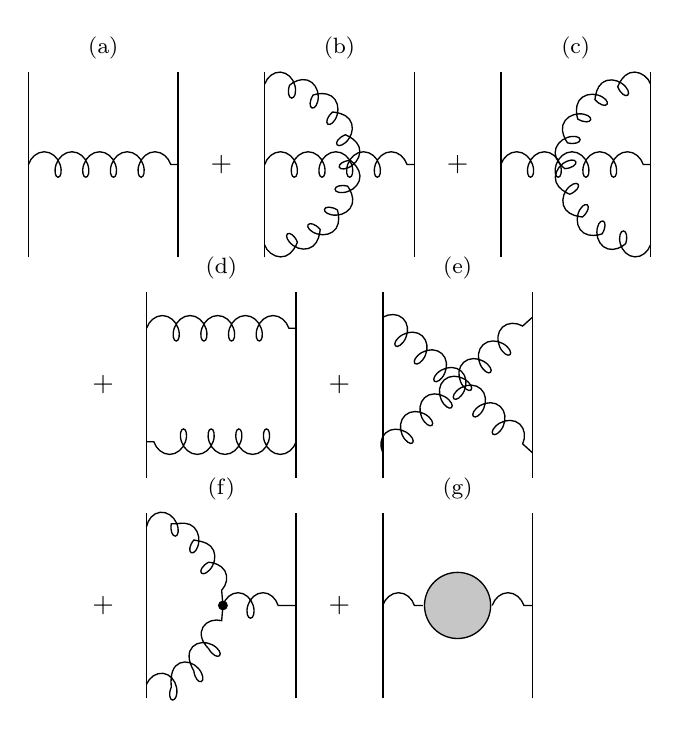
\begin{tikzpicture}[x=1cm,y=1cm,baseline=-.45ex]
  % Upper row: direct exchange and the two static-source self-energies.
  \BanksNPanel{0}{2.80}\BanksNPanel{3}{2.80}\BanksNPanel{6}{2.80}
  \BanksNHorizontal{0}{2.80}
  \BanksNHorizontal{3}{2.80}\BanksNArchLeft{3}{2.80}
  \BanksNHorizontal{6}{2.80}\BanksNArchRight{6}{2.80}

  % Middle row: the ladder and the crossed ladder.
  \BanksNPanel{1.5}{0}\BanksNPanel{4.5}{0}
  \BanksNHorizontal{1.5}{.72}\BanksNHorizontalUp{1.5}{-.72}
  \BanksNCross{4.5}{0}

  % Lower row: the triple-gluon vertex and the self-energy insertion.
  \BanksNPanel{1.5}{-2.80}\BanksNPanel{4.5}{-2.80}
  \BanksNTriple{1.5}{-2.80}\BanksNInsertion{4.5}{-2.80}

  \node at (0,4.28) {\footnotesize (a)};
  \node at (3,4.28) {\footnotesize (b)};
  \node at (6,4.28) {\footnotesize (c)};
  \node at (1.5,1.48) {\footnotesize (d)};
  \node at (4.5,1.48) {\footnotesize (e)};
  \node at (1.5,-1.32) {\footnotesize (f)};
  \node at (4.5,-1.32) {\footnotesize (g)};

  \node at (1.5,2.80) {$+$};
  \node at (4.5,2.80) {$+$};
  \node at (0,0) {$+$};
  \node at (3,0) {$+$};
  \node at (0,-2.80) {$+$};
  \node at (3,-2.80) {$+$};
\end{tikzpicture}

  \caption{One-loop contributions to the potential.}
  \label{fig:9.9}
\end{figure}

% BANKS-SOURCE: pdf=193 print=183 kind=source-page
% BANKS-SOURCE: pdf=193 print=183 kind=figure id=9.10
\begin{figure}[htbp]
  \centering
  % BANKS-SOURCE: pdf=193 print=183 kind=figure id=9.10
% The shaded gluon self-energy blob and the six one-loop graphs (a)--(f)
% that make it up.  Everything is native TikZ.
\tikzset{
  BanksFLine/.style={line width=.5pt},
  BanksFGluon/.style={line width=.5pt,decorate,
    decoration={coil,aspect=.7,amplitude=3.6pt,segment length=#1}},
  BanksFGluon/.default=8pt,
  BanksFTip/.style={postaction={decorate},decoration={markings,
    mark=at position .52 with {\arrow{Latex[length=1.9mm,width=1.9mm]}}}},
}

% A straight gluon stub from (#1,#3) to (#2,#3).
\newcommand{\BanksFStub}[3]{%
  \draw[BanksFGluon=6.5pt] (#1,#3)--(#2,#3);
}

% A longer straight gluon line, used for the two tadpole graphs.
\newcommand{\BanksFLong}[3]{%
  \draw[BanksFGluon=8.5pt] (#1,#3)--(#2,#3);
}

\newcommand{\BanksFDot}[2]{\fill (#1,#2) circle (.05);}

% Lens-shaped one-loop bubble between vertices at (#1-.62,#2) and
% (#1+.62,#2).  #3 carries the line style (dashed for ghosts and scalars),
% and the loop runs counter-clockwise: arrow left on top, right below.
\newcommand{\BanksFBubble}[3]{%
  \draw[BanksFLine,#3,BanksFTip]
    (#1+.62,#2) .. controls (#1+.32,#2+.66) and (#1-.32,#2+.66) .. (#1-.62,#2);
  \draw[BanksFLine,#3,BanksFTip]
    (#1-.62,#2) .. controls (#1-.32,#2-.66) and (#1+.32,#2-.66) .. (#1+.62,#2);
  \BanksFDot{#1-.62}{#2}\BanksFDot{#1+.62}{#2}%
}

% The same bubble as a gluon loop: a rounded oval whose coils point inward.
\newcommand{\BanksFGluonBubble}[2]{%
  \draw[BanksFGluon=7pt]
    (#1-.62,#2) .. controls (#1-.62,#2+.70) and (#1+.62,#2+.70) .. (#1+.62,#2);
  \draw[BanksFGluon=7pt]
    (#1+.62,#2) .. controls (#1+.62,#2-.70) and (#1-.62,#2-.70) .. (#1-.62,#2);
  \BanksFDot{#1-.62}{#2}\BanksFDot{#1+.62}{#2}%
}

\resizebox{0.95\textwidth}{!}{%
\begin{tikzpicture}[x=1cm,y=1cm,baseline=-.45ex]

  %% ---- first row: the definition, plus graphs (a) and (b) --------------
  % shaded blob
  \BanksFStub{0}{.85}{2.55}
  \draw[fill=gray!35,line width=.5pt] (1.6,2.55) ellipse (.72 and .44);
  \BanksFStub{2.35}{3.2}{2.55}
  \BanksFDot{.85}{2.55}\BanksFDot{2.35}{2.55}
  \node at (3.62,2.55) {$=$};

  % (a) gluon loop
  \BanksFStub{4.1}{4.98}{2.55}
  \BanksFGluonBubble{5.6}{2.55}
  \BanksFStub{6.22}{7.1}{2.55}
  \node at (5.6,1.42) {\footnotesize (a)};

  \node at (7.5,2.55) {$+$};

  % (b) gluon tadpole: one vertex on a straight gluon line, coiled loop above
  \BanksFLong{7.95}{9.45}{2.55}
  \BanksFLong{9.45}{10.95}{2.55}
  \draw[BanksFGluon=8pt] (9.45,2.55) arc (270:-90:.45);
  \BanksFDot{9.45}{2.55}
  \node at (9.45,1.42) {\footnotesize (b)};

  %% ---- second row: (c) ghost loop and (d) fermion loop ------------------
  \node at (1.85,.35) {$+$};
  \BanksFStub{2.35}{3.23}{.35}
  \BanksFBubble{3.85}{.35}{dashed}
  \BanksFStub{4.47}{5.35}{.35}
  \node at (3.85,-.75) {\footnotesize (c)};

  \node at (5.72,.35) {$+$};
  \BanksFStub{6.2}{7.08}{.35}
  \BanksFBubble{7.7}{.35}{}
  \BanksFStub{8.32}{9.2}{.35}
  \node[anchor=north] at (7.02,.12) {$\mathrm{R_F}$};
  \node[anchor=north] at (8.38,.12) {$\mathrm{R_F}$};
  \node at (7.7,-.75) {\footnotesize (d)};

  %% ---- third row: (e) scalar loop and (f) scalar tadpole ----------------
  \node at (2.35,-1.85) {$+$};
  \BanksFStub{2.85}{3.73}{-1.85}
  \BanksFBubble{4.35}{-1.85}{dashed}
  \BanksFStub{4.97}{5.85}{-1.85}
  \node[anchor=north] at (3.67,-2.08) {$\mathrm{R_S}$};
  \node[anchor=north] at (5.03,-2.08) {$\mathrm{R_S}$};
  \node at (4.35,-2.95) {\footnotesize (e)};

  \node at (6.25,-1.85) {$+$};
  \BanksFLong{6.75}{8.25}{-1.85}
  \BanksFLong{8.25}{9.75}{-1.85}
  \draw[BanksFLine,dashed,
        postaction={decorate},decoration={markings,
          mark=at position .25 with {\arrow{Latex[length=1.9mm,width=1.9mm]}}}]
    (8.65,-1.45) arc (0:360:.40);
  \BanksFDot{8.25}{-1.85}
  \node[anchor=north] at (8.25,-2.02) {$\mathrm{R_S}$};
  \node at (8.25,-2.95) {\footnotesize (f)};
\end{tikzpicture}%
}

  \caption{One-loop contributions to gluon vacuum polarization.}
  \label{fig:9.10}
\end{figure}

% BANKS-SOURCE: pdf=193 print=183 kind=prose
At fourth order in the coupling we have the seven graphs of Figure~\ref{fig:9.9},
the sixth of which vanishes in Feynman gauge. The gluon vacuum polarization,
denoted by a shaded oval, is computed from the graphs of Figure~\ref{fig:9.10}.

The first two graphs of Figure~\ref{fig:9.9} sum up to
% BANKS-SOURCE: pdf=193 print=183 kind=display
\[
\begin{aligned}
&\left(\frac12\right)^2g_0^4\mu^{2(4-d_{\mathrm{reg}})}
 \int\dd x_1\,\dd x_2\,\dd x_3\,
 D(x_1-x_3)D(x_2-x_4)\\[-2pt]
&\quad\times\operatorname{tr}\!\left[
 (T_R^aT_R^aT_R^bT_R^b)\theta(t_1-t_2)\theta(t_3-t_4)
 +(T_R^aT_R^bT_R^aT_R^b)\theta(t_1-t_2)\theta(t_4-t_3)\right].
\end{aligned}
\]
All $x_i$ variables are integrated over the full Wilson loop, from $-T/2$ to
$T/2$ at $R$ and then back again at the origin (we neglect the horizontal
sections of the loop because they don't give contributions that grow like
powers of $T$). The factor of $(1/2)^2$ eliminates double counting. The
$\theta$ functions refer to ordering around the Wilson loop. The first
contribution comes from the graph where the internal gluon lines do not cross
each other when all lines are drawn inside the loop.

If, in Figure~\ref{fig:9.9}(e), we write
% BANKS-SOURCE: pdf=193 print=183 kind=display
\[
  \operatorname{tr}(T_R^aT_R^bT_R^aT_R^b)
  =\operatorname{tr}(T_R^aT_R^aT_R^bT_R^b)
  +\frac12\operatorname{tr}[T_R^a,T_R^b]^2,
\]
then we can combine the first term with the graph of Figure~\ref{fig:9.9}(d)
to get precisely the square of the second-order result. The novel term thus
has the form
% BANKS-SOURCE: pdf=193 print=183 kind=display
\[
\begin{aligned}
&\left(\frac12\right)^2g_0^4\mu^{2(4-d_{\mathrm{reg}})}
 \int\dd x_1\,\dd x_2\,\dd x_3\,
 D(x_1-x_2)D(x_3-x_4)\\[-2pt]
&\quad\times\operatorname{tr}\!\left[
 [T_R^a,T_R^b]^2\theta(t_1-t_3)\theta(t_4-t_3)\right].
\end{aligned}
\]
The group-theory factor here gives $-f^{abc}f^{abc}D(R)=-C_2(G)d_GD(R)$,
in terms of the second Casimir operator of the group, its dimension, and the
Dynkin index of the representation $R$.

There are three types of configurations of the $x_i$ that contribute to the
integral. If all $x_i$ are on either the upward- or the downward-going line,
then the integral has no $R$ dependence. It contributes to the self-energy of
the static sources, but not to the potential between them. If three $x_i$ are
on either the upward or the downward line, as

% BANKS-SOURCE: pdf=194 print=184 kind=source-page
shown in Figure~\ref{fig:9.9}(c), we get (note that there is a minus sign from
the orientations of the different integration variables)
% BANKS-SOURCE: pdf=194 print=184 kind=display
\[
  4\int\dd t_1\,\dd t_2\,\dd t_3\,\dd t_4\,
  \theta(t_2-t_3)\theta(t_3-t_1)D(t_1-t_2,\mathbf 0)D(t_3-t_4,\mathbf R).
\]
All the integrals here go from $-T/2$ to $T/2$ and the $\theta$ functions are
ordinary step functions. In DR, the Green functions are
% BANKS-SOURCE: pdf=194 print=184 kind=display
\[
\begin{aligned}
  D(t,\mathbf R)&=\int\frac{\dd^{d_{\mathrm{reg}}}p}{(2\pi)^{d_{\mathrm{reg}}}}
  \frac{\ee^{-\ii(tp_0+\mathbf p\cdot\mathbf R)}}{p_0^2+\mathbf p^2}\\
  &=\left(\frac{1}{2\sqrt\pi}\right)^{d_{\mathrm{reg}}}
  \int_0^\infty\dd\alpha\,\alpha^{-d_{\mathrm{reg}}/2}
  \ee^{-(t^2+R^2)/(4\alpha)}.
\end{aligned}
\]
The contribution from Figure~\ref{fig:9.9}(b) is similar. The two kinds of
$R$-dependent contributions (Figures~\ref{fig:9.9}(b) and (c) and the
commutator term in Figure~\ref{fig:9.9}(e)) have equal group-theoretic factors,
since they are really part of the same topological configuration of the
Wilson-loop diagrams, distinguished only by the fact that we have chosen to
put part of the loop at infinity. The differences between them come from
$R$ dependence of the propagators, and the relative minus sign from the
orientation of the static line. Their sum is proportional to
$(t_{ij}\equiv t_i-t_j)$:
% BANKS-SOURCE: pdf=194 print=184 kind=display
\[
\begin{aligned}
T\Big[&\int\dd t_{23}\,\dd t_{21}\,\dd t_{34}\,
 \theta(t_{23})\theta(t_{21}-t_{23})
 \ee^{-\left(\frac{t_{21}^2}{4\alpha}+\frac{t_{34}^2}{4\beta}\right)}\\
&-\int\dd t_{31}\,\dd t_{21}\,\dd t_{34}\,
 \theta(t_{31})\theta(t_{21}-t_{31}+t_{34})
 \ee^{-\left(\frac{t_{21}^2+R^2}{4\alpha}
             +\frac{t_{34}^2+R^2}{4\beta}\right)}\Big].
\end{aligned}
\]
This must be integrated over $\alpha$ and $\beta$, with weight
$(\alpha\beta)^{-d_{\mathrm{reg}}/2}$.

In the first integral, we do the integral over $t_{23}$ to get a factor of
$t_{21}$. The latter variable is constrained to be positive. The rest of the
integral is a product of decoupled Gaussians and gives us a factor
$4\sqrt{\pi\alpha^2\beta}$. In the second integral we integrate over $t_{31}$
to get a factor of $\theta(t_+)t_+$, where $t_\pm=t_{12}\pm t_{34}$. In terms
of these new variables we find the sum of contributions to the
Schwinger-parameter integrands of the two diagrams to be
% BANKS-SOURCE: pdf=194 print=184 kind=display
\[
\begin{aligned}
T\Big[&4\sqrt{\pi\alpha^2\beta}\,\ee^{-R^2/(4\beta)}\\[-2pt]
&-\int\dd t_+\,\dd t_-\,\theta(t_+)t_+
 \ee^{-(t_+^2+t_-^2+4R^2)\left(\frac{1}{16\alpha}+\frac{1}{16\beta}\right)}
 \ee^{-t_+t_-\left(\frac{1}{8\alpha}-\frac{1}{8\beta}\right)}\Big].
\end{aligned}
\]
We now do the Gaussian integral over $t_-$, followed by that over $t_+$. The
resulting sum of the two diagrams is
% BANKS-SOURCE: pdf=194 print=184 kind=display
\[
\begin{aligned}
 -&\frac{g_0^4\mu^{2(4-d_{\mathrm{reg}})}C_2(G)d_AD(R)}{2^{d_{\mathrm{reg}}}\pi^{d_{\mathrm{reg}}/2}}
 4\sqrt\pi\int\dd\alpha\,\dd\beta\,(\alpha\beta)^{-d_{\mathrm{reg}}/2}
 \ee^{-R^2/(4\beta)}\\[-2pt]
&\qquad\times\alpha\sqrt\beta
 \left(1-\ee^{-R^2/(4\alpha)}\sqrt{1+\frac{\beta}{\alpha}}\right).
\end{aligned}
\]

% BANKS-SOURCE: pdf=195 print=185 kind=source-page
The change of variables $\alpha=s(1-x)$, $\beta=sx$ gives
% BANKS-SOURCE: pdf=195 print=185 kind=equation id=9.4
\begin{equation}
\begin{aligned}
-&\frac{g_0^4\mu^{2(4-d_{\mathrm{reg}})}C_2(G)d_AD(R)}{2^{d_{\mathrm{reg}}}\pi^{d_{\mathrm{reg}}/2}}
 4\sqrt\pi\left(\frac{R^2}{4}\right)^{7/2-d_{\mathrm{reg}}}\\[-2pt]
&\quad\times\int\dd s\,\dd x\,s^{5/2-d_{\mathrm{reg}}}[x(1-x)]^{-d_{\mathrm{reg}}/2}
 \ee^{-1/[sx(1-x)]}\sqrt{x}
 \left(1-\ee^{-1/[s(1-x)]}\sqrt{\frac{1}{1-x}}\right).
\end{aligned}
\label{eq:9.4}
\end{equation}
As usual, divergences come from the limits of the Schwinger-parameter
integrals. Note, however, that the $s$ integral converges for small $s$. The
UV divergence comes from the region $x\sim1$, from which we get a pole at
$d_{\mathrm{reg}}=4$. It is probing the short-distance singularity of only a single
propagator. Indeed, we can do the $s$ integral exactly and obtain
% BANKS-SOURCE: pdf=195 print=185 kind=equation id=9.5
\begin{equation}
\begin{aligned}
-&\frac{g_0^4\mu^{2(4-d_{\mathrm{reg}})}C_2(G)d_AD(R)}{2^{d_{\mathrm{reg}}}\pi^{d_{\mathrm{reg}}/2}}
 4\sqrt\pi\,\Gamma\!\left(d_{\mathrm{reg}}-\frac72\right)
 \left(\frac{R^2}{4}\right)^{7/2-d_{\mathrm{reg}}}\\[-2pt]
&\quad\times\int\dd x\,x^{d_{\mathrm{reg}}/2-3}
 \left[(1-x)^{1-d_{\mathrm{reg}}/2}-(1-x)^{d_{\mathrm{reg}}/2-3}\right].
\end{aligned}
\label{eq:9.5}
\end{equation}
The integrals can be evaluated in terms of Euler beta functions, and the first
term has a pole at $d_{\mathrm{reg}}=4$, as a consequence of the singularity of its integrand
at $x=1$.

Next we compute the diagrams which correct the internal gauge-boson line. We
will do the computation in Feynman gauge and continue the loop expressions to
Minkowski space, retaining the $-\ii0$ prescription in each massless
denominator. In Problem 8.13 the reader will verify
that the answer for the full Wilson loop is the same in any covariant gauge.
The theory is invariant both under constant gauge transformations and under
BRST symmetry. The first of these tells us that the gauge-boson two-point
function is proportional to $\delta^{ab}$. Given this constraint, the BRST-
symmetry relation for the two-point function reduces to the same constraint as
that which we found in abelian gauge theory: the two-point function is
transverse. So we have
% BANKS-SOURCE: pdf=195 print=185 kind=display
\[
  \Pi_{\mu\nu}{}^{ab}(q)=
  (\delta_{\mu\nu}q^2-q_\mu q_\nu)\delta^{ab}\Pi(q^2).
\]
Our QED calculations have shown us that dimensional regularization preserves
BRST symmetry, so it is sufficient to calculate the trace of the diagrams,
which gives us $\delta^{ab}(d_{\mathrm{reg}}-1)q^2\Pi(q^2)$. The reader is urged to carry out
the full calculation of all components in a general covariant gauge, in order
to convince her/himself that the result is indeed transverse. In this exercise,
it will become apparent that individual graphs do not satisfy the Ward
identities. They are true only for the sum of graphs at a given order.

\BanksImplicitHook{I-CH09-020}

The graphs in Figures~\ref{fig:9.10}(d)--(f) involving fermions or scalars are
proportional to their values in QED. The square of the integer charge of the
fields is replaced by the Dynkin index
$\operatorname{tr}(T_R^aT_R^b)=D(R)\delta^{ab}$ for the, generally reducible,
representations of the gauge group in which these fields live. Thus, the
divergent part of the gauge-boson two-point functions from these diagrams is
% BANKS-SOURCE: pdf=195 print=185 kind=equation id=9.7
\begin{equation}
  \Pi_{F+S}{}^{\mu a\,\nu b}
  =\ii(q^2\eta^{\mu\nu}-q^\mu q^\nu)\delta^{ab}
  \left(-\frac{\alpha_G}{4\pi}\right)\mu^{d_{\mathrm{reg}}-4}
  \left[\frac23D(R_F)+\frac13D(R_S)\right]
  \Gamma\!\left(2-\frac {d_{\mathrm{reg}}}{2}\right).
\label{eq:9.7}
\end{equation}

% BANKS-SOURCE: pdf=196 print=186 kind=source-page
$\alpha_G$ is the analog of the fine-structure constant for the non-abelian
group $G$. We have done the computation for Weyl fermion fields in the
representation $R_F$. For parity-invariant gauge couplings to Dirac fields, we
should make the replacement $2/3\to4/3$. Similarly, our computation was done
for complex scalar fields. If some of the irreducible components of $R_S$ are
real, and we have only one real field in this irreducible representation, the
corresponding contribution is smaller by a factor of $1/2$. The reader should
remember these factors of two when applying the above formula to specific
theories.

The pure gauge-theory contribution to the gauge-boson two-point function
consists of three graphs, Figures~\ref{fig:9.10}(a)--(c). The most complicated
is the one involving triple gauge-boson vertices. It has the form
% BANKS-SOURCE: pdf=196 print=186 kind=equation id=9.8
\begin{equation}
  \Pi_{V_1}{}^{\mu a\,\nu b}
  =\frac{(-\ii)^2g_0^2\mu^{d_{\mathrm{reg}}-4}}{2}f^{acd}f^{bcd}
  \int\frac{\dd^{d_{\mathrm{reg}}}p}{(2\pi)^{d_{\mathrm{reg}}}}
  \frac{N^{\mu\nu}}{(p^2-\ii0)((p+q)^2-\ii0)}.
\label{eq:9.8}
\end{equation}
where the numerator factor is
% BANKS-SOURCE: pdf=196 print=186 kind=display
\[
\begin{aligned}
N^{\mu\nu}={}&\left[\eta^{\mu\rho}(q-p)^\alpha
 +\eta^{\rho\alpha}(2p+q)^\mu-\eta^{\alpha\mu}(p+2q)^\rho\right]\\
&\quad\times\left[\delta_\rho^\nu(p-q)_\alpha
 -\eta_{\rho\alpha}(2p+q)^\nu+\delta_\alpha^\nu(p+2q)_\rho\right].
\end{aligned}
\]
The overall factor of $1/2$ is a symmetry factor. The trace of the numerator is
% BANKS-SOURCE: pdf=196 print=186 kind=display
\[
  N^\mu{}_{\mu}=-6(d_{\mathrm{reg}}-1)(p^2+q^2+pq).
\]
The group-theory factor can be written in terms of the second Casimir operator,
% BANKS-SOURCE: pdf=196 print=186 kind=display
\[
  f^{acd}f^{bcd}=\delta^{ab}C_2(G).
\]
Thus
% BANKS-SOURCE: pdf=196 print=186 kind=equation id=9.9
\begin{equation}
  \Pi_{V_1\mu}{}^{\mu ab}
  =3(d_{\mathrm{reg}}-1)g_0^2\mu^{d_{\mathrm{reg}}-4}\delta^{ab}C_2(G)
  \int\frac{\dd^{d_{\mathrm{reg}}}p}{(2\pi)^{d_{\mathrm{reg}}}}
  \frac{p^2+q^2+pq}{(p^2-\ii0)((p+q)^2-\ii0)}.
\label{eq:9.9}
\end{equation}
The diagram of Figure~\ref{fig:9.10}(b) is given by
% BANKS-SOURCE: pdf=196 print=186 kind=equation id=9.10
\begin{equation}
\begin{aligned}
  \Pi_{V_2}{}^{\mu a\,\nu b}={}&
  \frac{(-\ii)^2g_0^2\mu^{d_{\mathrm{reg}}-4}}{2}
  \int\frac{\dd^{d_{\mathrm{reg}}}p}{(2\pi)^{d_{\mathrm{reg}}}}
  \frac{\delta^{dc}\eta^{\alpha\beta}}{p^2-\ii0}\\
  &\quad\times\big[ f^{abe}f^{cde}
  (\eta^{\mu\alpha}\eta^{\nu\beta}-\eta^{\nu\alpha}\eta^{\beta\mu})\\
  &\qquad\quad+f^{ace}f^{bde}
  (\eta^{\mu\nu}\eta^{\alpha\beta}-\eta^{\mu\alpha}\eta^{\beta\nu})\\
  &\qquad\quad+f^{ade}f^{bce}
  (\eta^{\mu\nu}\eta^{\alpha\beta}-\eta^{\nu\alpha}\eta^{\beta\mu})\big].
\end{aligned}
\label{eq:9.10}
\end{equation}
We can reduce the group-theory factors and find that
% BANKS-SOURCE: pdf=196 print=186 kind=equation id=9.11
\begin{equation}
  \Pi_{V_2}{}^{\mu a\,\nu b}
  =-C_2(G)(d_{\mathrm{reg}}-1)g_0^2\mu^{d_{\mathrm{reg}}-4}
  \int\frac{\dd^{d_{\mathrm{reg}}}p}{(2\pi)^{d_{\mathrm{reg}}}}
  \frac{\delta^{ab}\eta^{\mu\nu}(p^2+q^2+2pq)}{(p^2-\ii0)((p+q)^2-\ii0)}.
\label{eq:9.11}
\end{equation}
Finally, we have the diagram in Figure~\ref{fig:9.10}(c), with the ghost loop,
% BANKS-SOURCE: pdf=196 print=186 kind=equation id=9.12
\begin{equation}
  \Pi_{V_3}{}^{\mu a\,\nu b}
  =-(\ii)^2g_0^2\mu^{d_{\mathrm{reg}}-4}f^{dac}f^{cbd}
  \int\frac{\dd^{d_{\mathrm{reg}}}p}{(2\pi)^{d_{\mathrm{reg}}}}
  \frac{(p+q)^\mu p^\nu}{(p^2-\ii0)((p+q)^2-\ii0)}.
\label{eq:9.12}
\end{equation}

% BANKS-SOURCE: pdf=197 print=187 kind=source-page
where we note the absence of a symmetry factor and a minus sign, coming from
the fact that the ghosts are complex scalar fermions. In contrast to physical
scalars, there is no quartic coupling between the ghosts and the gauge bosons
in the gauge we are using. The group-theory factor in this diagram is
$-C_2(G)\delta^{ab}$.

The sum of these three diagrams gives
% BANKS-SOURCE: pdf=197 print=187 kind=display
\[
  \Pi_\mu{}^{\mu ab}=g_0^2\mu^{d_{\mathrm{reg}}-4}\delta^{ab}C_2(G)
  \int\frac{\dd^{d_{\mathrm{reg}}}p}{(2\pi)^{d_{\mathrm{reg}}}}
  \frac{N(d_{\mathrm{reg}},x,p,q)}{(p^2-\ii0)((p+q)^2-\ii0)},
\]
where
% BANKS-SOURCE: pdf=197 print=187 kind=display
\[
  N(d_{\mathrm{reg}},x,p,q)=3(d_{\mathrm{reg}}-1)(p^2+q^2+pq)
  -d_{\mathrm{reg}}(d_{\mathrm{reg}}-1)(p^2+q^2+2pq)-(p^2+pq).
\]

We now introduce a Feynman parameter $x$ to simplify the denominator, and
define $r=p-xq$, $U=x(1-x)q^2$. We can then discard terms in the numerator
linear in $r$ and write it as
% BANKS-SOURCE: pdf=197 print=187 kind=display
\[
  -(d_{\mathrm{reg}}-2)^2(r^2+x^2q^2)
  +(2d_{\mathrm{reg}}^2-5d_{\mathrm{reg}}+4)xq^2.
\]
Note that the term in the numerator quadratic in the integration variable is
multiplied by $(d_{\mathrm{reg}}-2)^2$. The integral over this term will give rise to a pole at
$d_{\mathrm{reg}}-2$, which is the signal of a quadratic divergence in DR. The fact that it is
multiplied by $d_{\mathrm{reg}}-2$ indicates that this pole is absent and there is no
quadratic divergence, and thus no divergent gauge-boson mass.

As usual, we do the integrals by analytically continuing to Euclidean space. I
take the opportunity to record here the Minkowski-space values of two
dimensionally regulated integrals which are obtained by this method:
% BANKS-SOURCE: pdf=197 print=187 kind=display
\[
  \int\frac{\dd^{d_{\mathrm{reg}}}p}{(2\pi)^{d_{\mathrm{reg}}}}
  \frac{1}{(p^2+U-\ii0)^n}
  =\frac{(-1)^n\ii}{2^{d_{\mathrm{reg}}}\pi^{d_{\mathrm{reg}}/2}}
  \frac{\Gamma(n-d_{\mathrm{reg}}/2)}{\Gamma(n)}
  \left(\frac{1}{U}\right)^{n-d_{\mathrm{reg}}/2}
\]
and
% BANKS-SOURCE: pdf=197 print=187 kind=display
\[
  \int\frac{\dd^{d_{\mathrm{reg}}}p}{(2\pi)^{d_{\mathrm{reg}}}}
  \frac{p^\mu p^\nu}{(p^2+U-\ii0)^n}
  =\frac{(-1)^{n-1}\ii\eta^{\mu\nu}}{2^{d_{\mathrm{reg}}+1}\pi^{d_{\mathrm{reg}}/2}}
  \frac{\Gamma(n-d_{\mathrm{reg}}/2-1)}{\Gamma(n)}
  \left(\frac{1}{U}\right)^{n-d_{\mathrm{reg}}/2-1}.
\]
The reader should note how the argument of the numerator Euler function
corresponds to the power of $U$. Once one has understood the methods of
Euclidean field theory, it is often convenient to just remember such a table of
effective Minkowski integrals.

\BanksImplicitHook{I-CH09-021}

The reader is asked to complete the computation of the renormalized static
potential $V(R)$ in Problem 9.10. He/she will find that the $\beta$ function for
the Yang--Mills coupling is given by
% BANKS-SOURCE: pdf=197 print=187 kind=display
\[
  \beta(g)=-\frac{g^3}{16\pi^2}
  \left(\frac{11}{3}C_2(G)-\frac{2}{3}D(R_F)-\frac{1}{3}D(R_S)\right).
\]
$C_2(G)$ is the quadratic Casimir invariant of the adjoint representation, and
$D(R)$ is the Dynkin index of the representation $R$. We have done the
computation for Weyl fermions (Dirac fermions will give an extra factor of two)
and complex scalars (real scalars are possible for real components of $R_S$ and
give an extra factor of $\tfrac12$). As long as there are not too many matter
fields, the non-abelian gauge coupling is marginally irrelevant or
asymptotically free \cite{banks-ref-113,banks-ref-114,banks-ref-115,banks-ref-116,banks-ref-117,banks-ref-118}.
A definition of the coupling in terms of the potential is

% BANKS-SOURCE: pdf=198 print=188 kind=source-page
manifestly independent of the gauge parameter. On the other hand, Problem 9.9
shows that the first two terms in the $\beta$ function are the same for all
renormalization schemes whose couplings are related by power-series expansions.
Thus the first two terms of the $\beta$ function are universal,
scheme-independent, and gauge-invariant. A general definition of the gauge
coupling will not have a $\kappa$-independent $\beta$ function beyond two loops.

The static potential in a massless gauge theory will satisfy the RG equation
% BANKS-SOURCE: pdf=198 print=188 kind=display
\[
  (\mu\partial_\mu+\beta(g)\partial_g)V(R,g,\mu)=0,
\]
while dimensional analysis implies that
% BANKS-SOURCE: pdf=198 print=188 kind=display
\[
  (\mu\partial_\mu-R\partial_R)V=V.
\]
Together, these equations imply that
% BANKS-SOURCE: pdf=198 print=188 kind=display
\[
  V=-\frac{g_0^2C_2(R)}{4\pi R}.
\]
The potential is essentially the Coulomb potential, multiplied by the running
coupling at scale $1/R$. In perturbation theory, this relation arises because
all non-scale-invariant $R$ dependence is a function of $R\mu$, but all $\mu$
dependence comes through the bare coupling and survives in the physical limit
$D=4$ only
when it multiplies a pole. The RG equation implies that the $k$th loop term in
perturbation theory will be a $k$th-order polynomial in $\ln(\mu R)$.
